%%%%%%%%%%%%%%%%%%%%%%%%%%%%%%%%%%%%%%%%%%%%%%%%%%%%%%%%%%%%%%%
%
% Welcome to Overleaf --- just edit your article on the left,
% and we'll compile it for you on the right. If you give 
% someone the link to this page, they can edit at the same
% time. See the help menu above for more info. Enjoy!
%
%%%%%%%%%%%%%%%%%%%%%%%%%%%%%%%%%%%%%%%%%%%%%%%%%%%%%%%%%%%%%%%
%
% For more detailed article preparation guidelines, please see:
% http://f1000research.com/author-guidelines

\documentclass[10pt,a4paper,twocolumn]{article}
\usepackage{arm_styles}

%% Default: numerical citations
\usepackage[numbers]{natbib}
\usepackage{subfigure}
\usepackage{subcaption}

%% Uncomment this lines for superscript citations instead
% \usepackage[super]{natbib}

%% Uncomment these lines for author-year citations instead
% \usepackage[round]{natbib}
% \let\cite\citep

\begin{document}

\title{\textit{Do human prototypicality ratings correlate with neural network categorization?}}
\author{Akif Berber, Lisa Goerke, Arianne van de Griend, Germonda Mooij, Ralitsa Spasova, Kai Standvoß}
%\author[3]{}
%\author[4]{Germonda Mooij}
%\author[5]{Ralitsa Spasova}
%\author[6]{Kai Standvoß}
%\affil[1]{}
%\affil[2]{}


\maketitle
\thispagestyle{fancy}

\begin{abstract}

This study rocks

\end{abstract}

\section*{Introduction}
Individual

\section*{Methods}
\subsection*{Neural network study}
500 Images of each category, 20 categories, 1000 categorylabels (ImageNet)
Weights from \cite{simonyan2014very}
For all 10,000 images the percentage of each of the 1000 labels is computed.
\subsection*{Baseline study}
\subsection*{Human study}
For the human experiment, a questionnaire is designed to measure human prototypicality ratings. The questionnaire consists of an introduction informing the participants about their rights and asking for their consent. Following this, the participants' demographic data, including age, gender and home-country, is accessed and participants are asked, if their color vision is impaired. Two example questions are presented to familiarize participants with the task. The images shown do belong to a category (envelopes) which is not presented in the actual study. For the actual study, 11 categories are selected (TODO based on what) as shown in table \ref{tab:cat_per}. For each category, all images are sorted after the classifications made by the neural network, and 10 images are chosen evenly over this distribution. The resulting range of network classification percentages can also be found in table \ref{tab:cat_per}. The 110 images are then randomized. Participants are asked for every image to rate its typicality on a Likert scale. In a Likert Scale participants give a quantitative value to a question based on a certain dimension, mostly the level of agreement/disagreement to that statement or question. In this questionnaire, the level of typicality was accessed. There are 7 answer options from the number one, representing "less typical", to seven, representing "very typical". The questionnaire ends with the possibility to give a free text comment about the survey.

To avoid learning effects, three differently randomized versions of the questionnaire are created and evenly distributed among participants (randomization 1: 35 participants, randomization 2: 13 participants, randomization 3: 26 participants) 
\begin{table}[ht]
\begin{center}
\begin{tabular}{l r r}
\multirow{3}{*}{Category} & Minimum & Maximum \\
 & percentage &  percentage \\
 & network & network \\
\hline
Volcano & 0.0001 & 100 \\
House & 0.1\hphantom{001} & 81\\
Airplane & 0.1\hphantom{001} & 95 \\
Car & 1\hphantom{.0001} & 93 \\
Coffee mug & 1\hphantom{.0001} & 98 \\
Teapot & 3\hphantom{.0001} & 97 \\
Table & 13\hphantom{.0001} & 96 \\
Church & 15\hphantom{.0001} & 78 \\
Castle & 31\hphantom{.0001} & 100 \\
Fruit & 55\hphantom{.0001} & 99 \\
Dog & 93\hphantom{.0001} & 100
\end{tabular}
\end{center}
\caption{TODO}
\label{tab:cat_per}
\end{table}

\section*{Results}
\subsection*{Neural network study}
\subsection*{Baseline study}
\subsection*{Human study}
For the human experiment, the designed questionnaire is distributed among various target groups. In total, 74 participants (35 male, 38, female, 1 other) answer to the questionnaire. Participant's age ranges from 12 to 56 ($\mu=27$, $\sigma^2=9.6$).

\begin{table}[ht]
\begin{center}
\begin{tabular}{l r l}
\multirow{3}{*}{Category} & Pearson's & \multirow{3}{*}{p-values} \\
 & correlation &   \\
 & coefficient &  \\
\hline
Fruit & 0.6586 & \textbf{0.0384} \\
Church & 0.1018 & 0.7795 \\
Dog & 0.2868 & 0.4218 \\
Houses & 0.5783 & 0.0799 \\
Teapot & 0.3454 & 0.3284 \\
Table & 0.0652 & 0.858 \\
Airplane & -0.2698 & 0.451 \\
Coffee mug & 0.3791 & 0.28 \\
Volcano & -0.3819 & 0.2762 \\
Castle & 0.1159 & 0.7499 \\
Car & 0.3516 & 0.3190\\
\end{tabular}
\end{center}
\caption{TODO}
\label{tab:pearsons}
\end{table}

\begin{figure*}
\begin{center}
\begin{subfigure}[t]
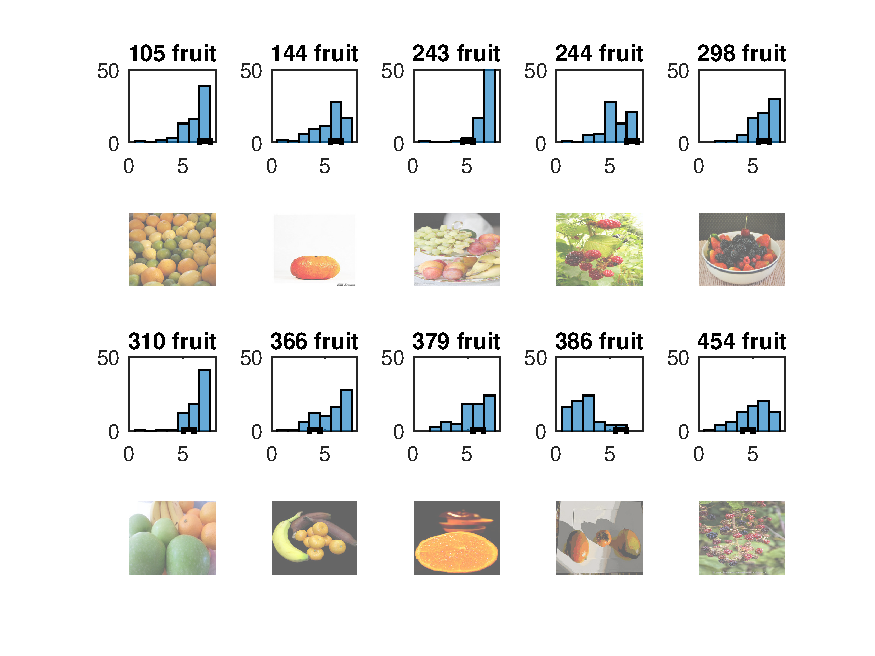
\includegraphics[width=\textwidth]{fruit_hist.pdf}
\caption{TODO}
\end{subfigure}
\begin{subfigure}[t]
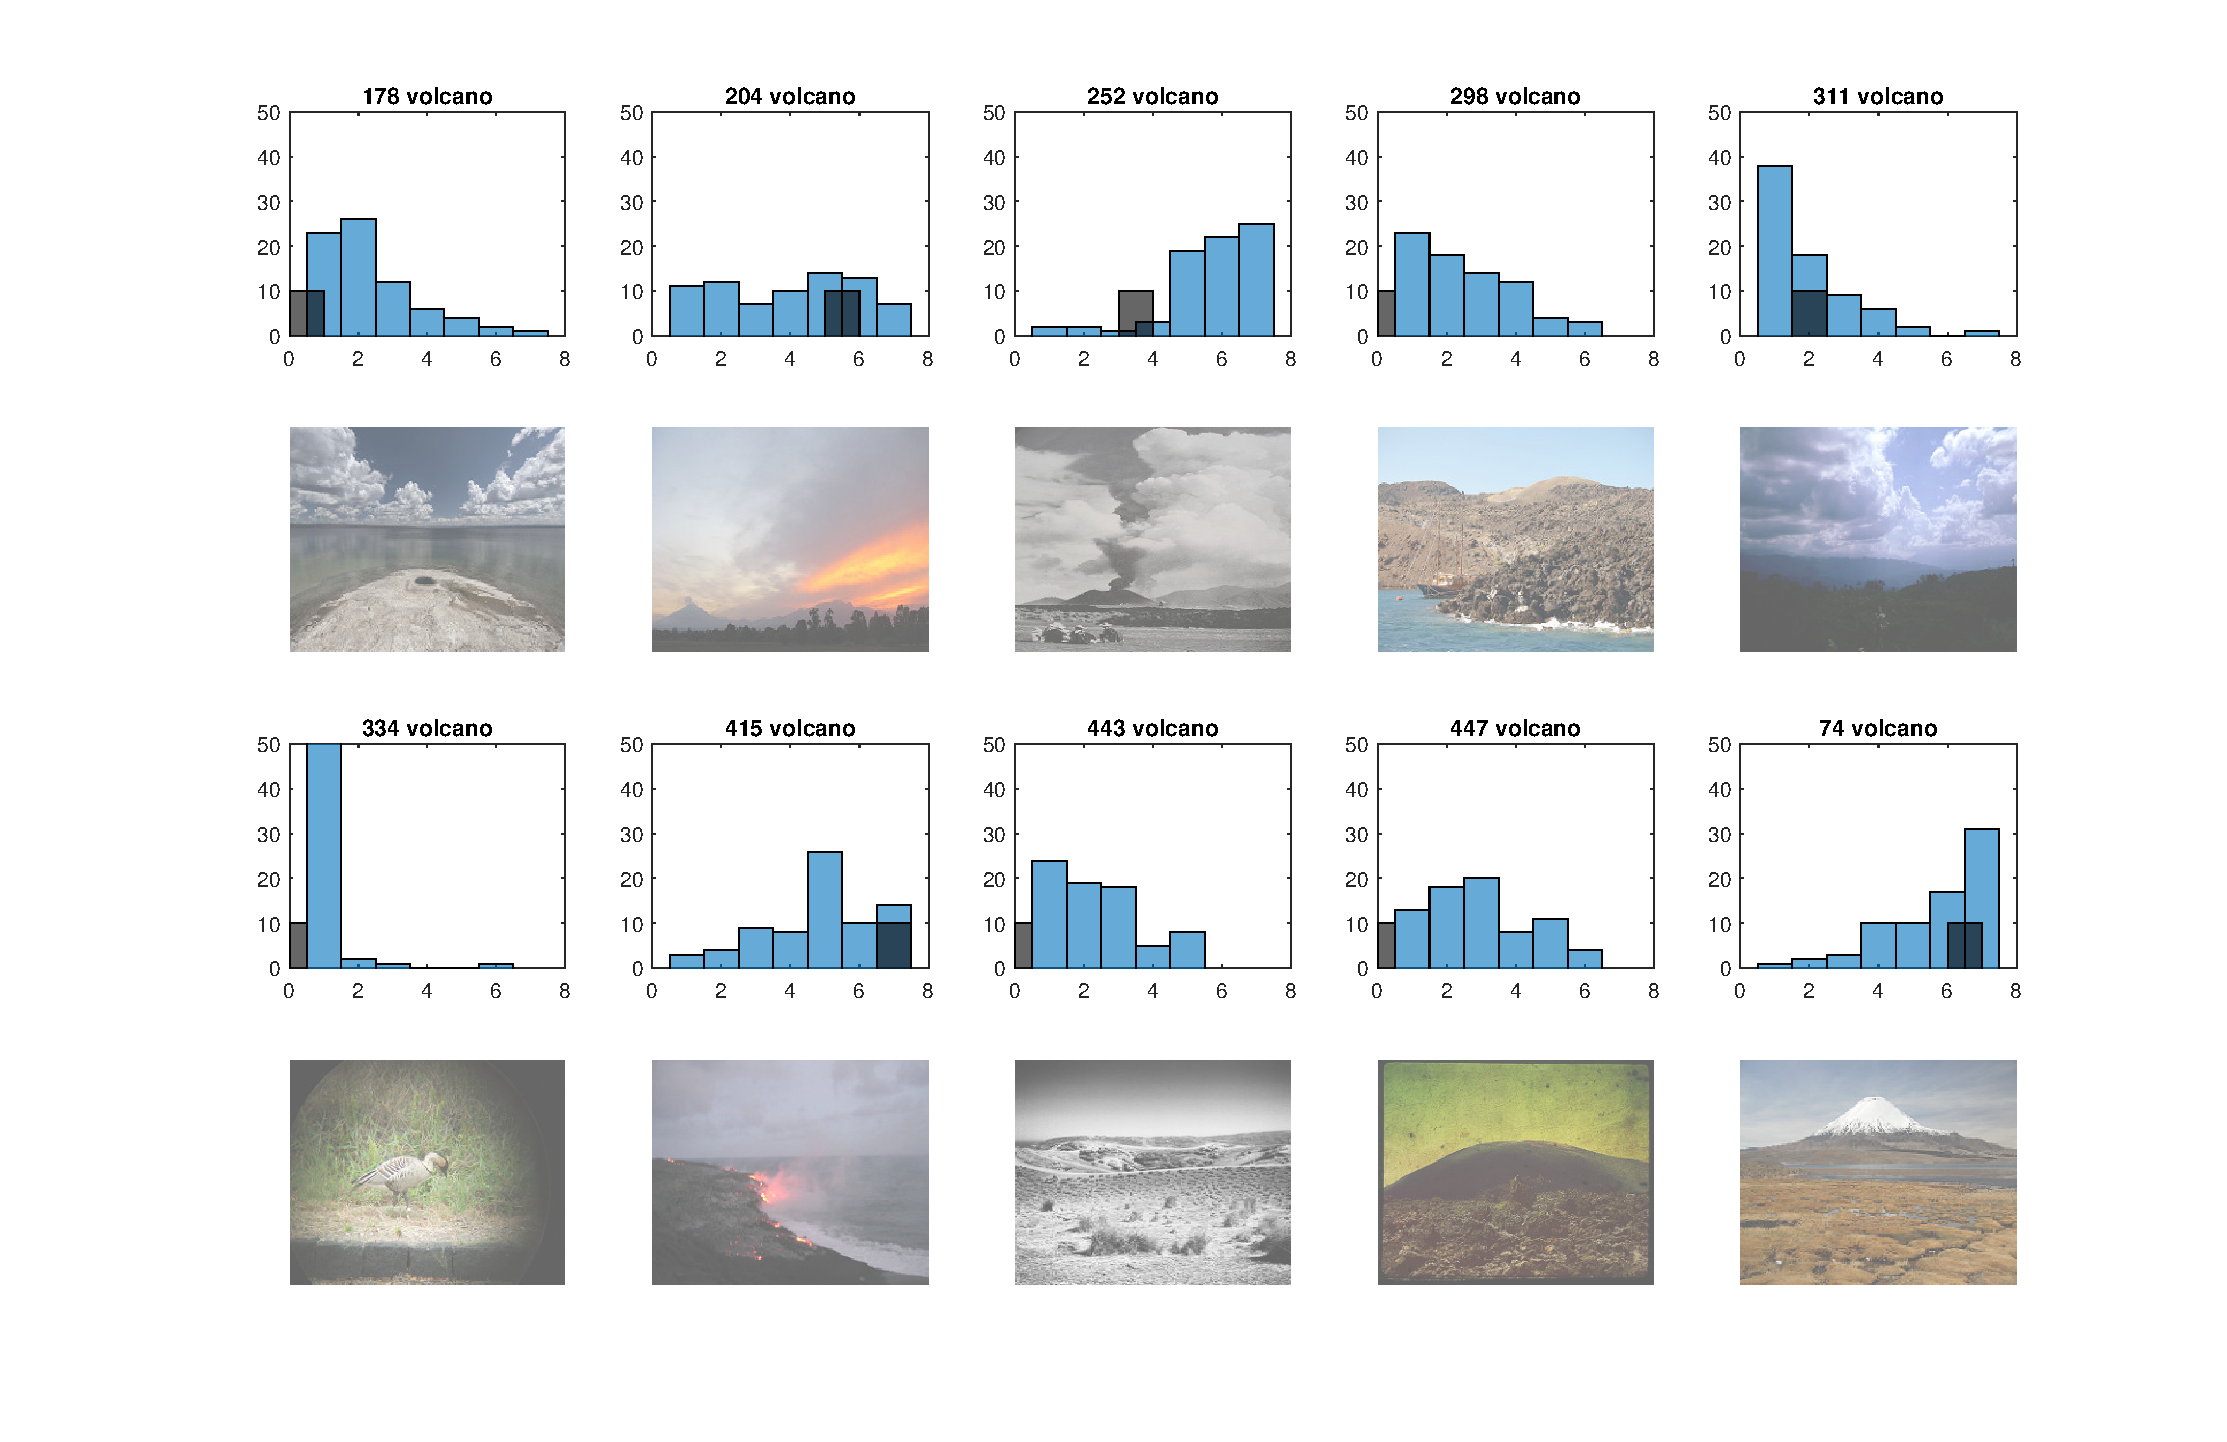
\includegraphics[width=\textwidth]{volcano_hist.pdf}
\caption{TODO}
\end{subfigure}
\hfill
\begin{subfigure}[t]
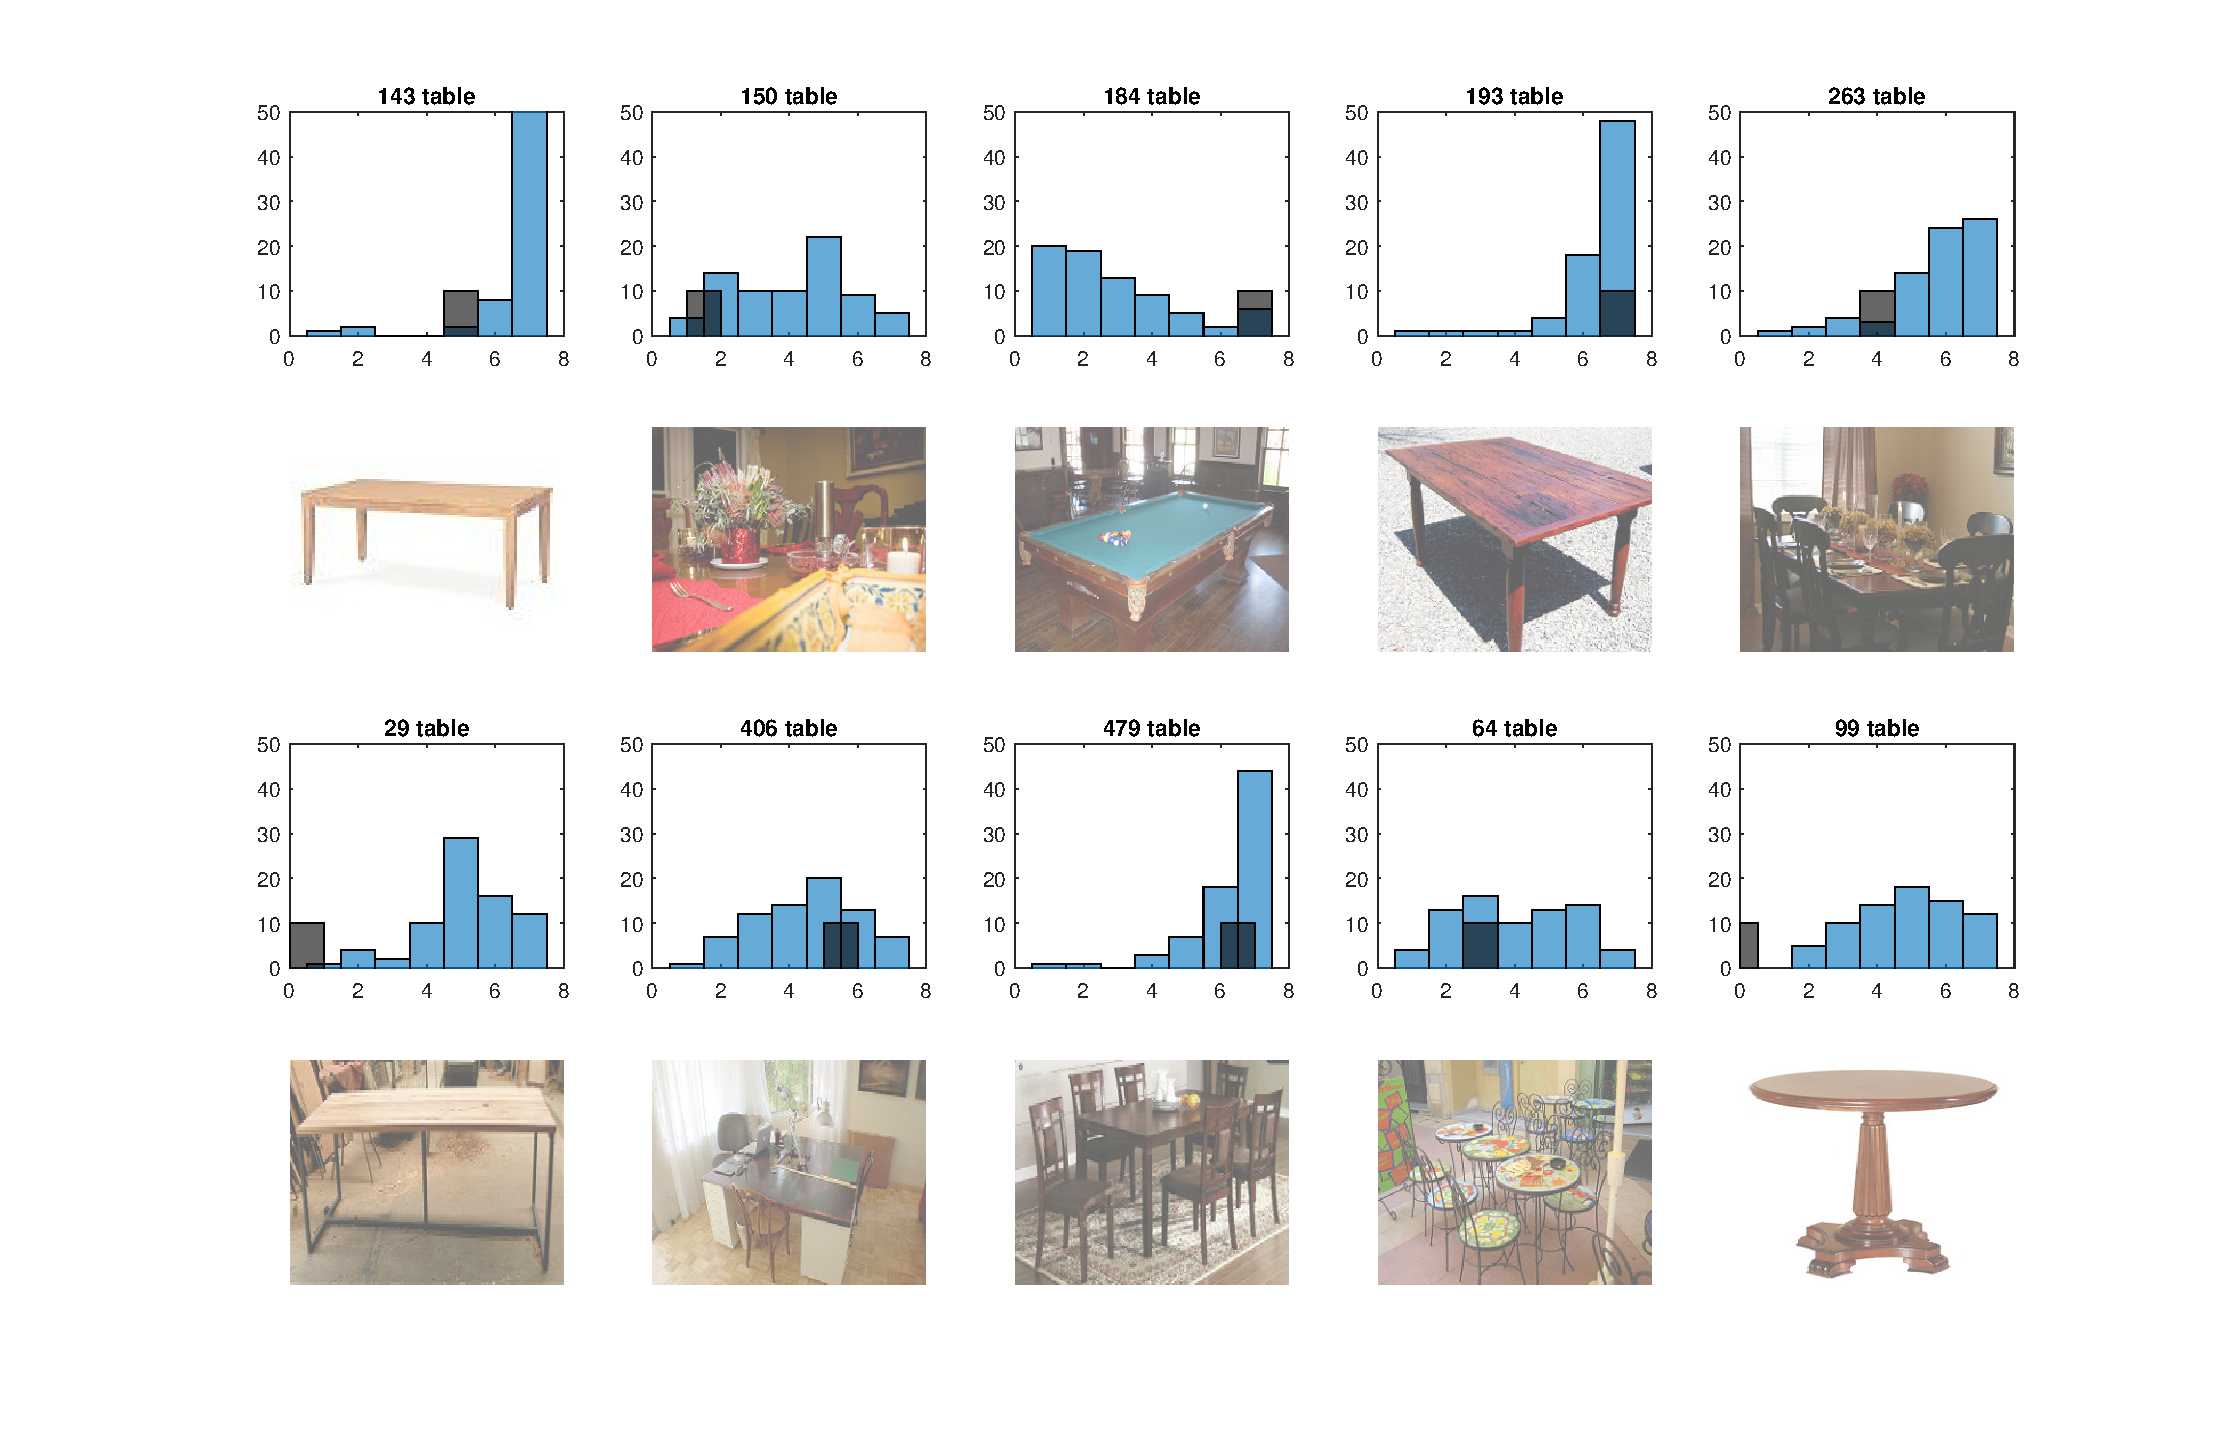
\includegraphics[width=\textwidth]{table_hist.pdf}
\caption{TODO}
\end{subfigure}
\end{center}
\caption{TODO}
\label{fig:fruit_hist}
\end{figure*}
                        
\section*{Discussion}
Individual

\section*{Conclusions}
Individual

{\small\bibliographystyle{unsrtnat}

\nocite{rosch1975family}
\nocite{lake2015deep}
\nocite{minda2002comparing}
\nocite{smith1998prototypes}
\nocite{reed1972pattern}
\nocite{rosch1999principles}
\nocite{posner1968genesis}

\bibliography{sources}}

\end{document}